% Top-align figures that land alone on a float page (default vertically centers them)
\makeatletter
\setlength{\@fptop}{0pt}
\makeatother

\begin{appendix} %Anhang
\section{Appendix}
\label{sec:appendix}

\subsection{Model Prices During the Experiment Window}
\label{app:model-prices}

The per-run costs in the experiment log are computed as native token counts times the model's
advertised OpenRouter price at run time. \Cref{tab:recovered-rates} lists the rates in effect.
Only GLM-5.2 changed price during the window. The open-weight models (GLM-5.2, DeepSeek-V3.2,
Ministral-14B) are served by multiple competing providers on OpenRouter, so their advertised
price is whatever the cheapest provider currently charges and can move at any time.

\begin{table}[htbp]
\centering
\small
\begin{tabular}{@{}llrr@{}}
\toprule
\textbf{Model} & \textbf{Period} & \textbf{Input \$/Mtok} & \textbf{Output \$/Mtok} \\
\midrule
anthropic/claude-opus-4.8    & whole window          & 5.00   & 25.00 \\
openai/gpt-5.5               & whole window          & 5.00   & 30.00 \\
qwen/qwen3.7-max             & whole window          & 1.25   & 3.75  \\
deepseek/deepseek-v3.2       & whole window          & 0.2288 & 0.3432 \\
mistralai/ministral-14b-2512 & whole window          & 0.20   & 0.20  \\
z-ai/glm-5.2                 & 2026-06-29            & 0.95   & 3.00  \\
z-ai/glm-5.2                 & 2026-06-30            & 0.94   & 3.00  \\
z-ai/glm-5.2                 & 2026-07-02 -- 07-03   & 0.93   & 3.00  \\
\bottomrule
\end{tabular}
\caption{OpenRouter list prices per million tokens during the experiment window.}
\label{tab:recovered-rates}
\end{table}

\subsection{Additional Experiment Figures}
\label{app:extra-figures}

\Cref{fig:invalid-commands} shows the malformed device commands as totals over the five runs of
each scenario--model pair. \Cref{fig:scenario-ttd} breaks the time to a correct diagnosis down
to scenario level (correct, completed runs only). A missing row means the model never solved
that scenario. \Cref{fig:wall-clock-distribution} shows the wall-clock time of all 300 runs,
including wrong diagnoses and DNFs. The runs stopped by the time limit form the clusters at
the 600-second cap.

\begin{figure}[htbp]
\begin{center}
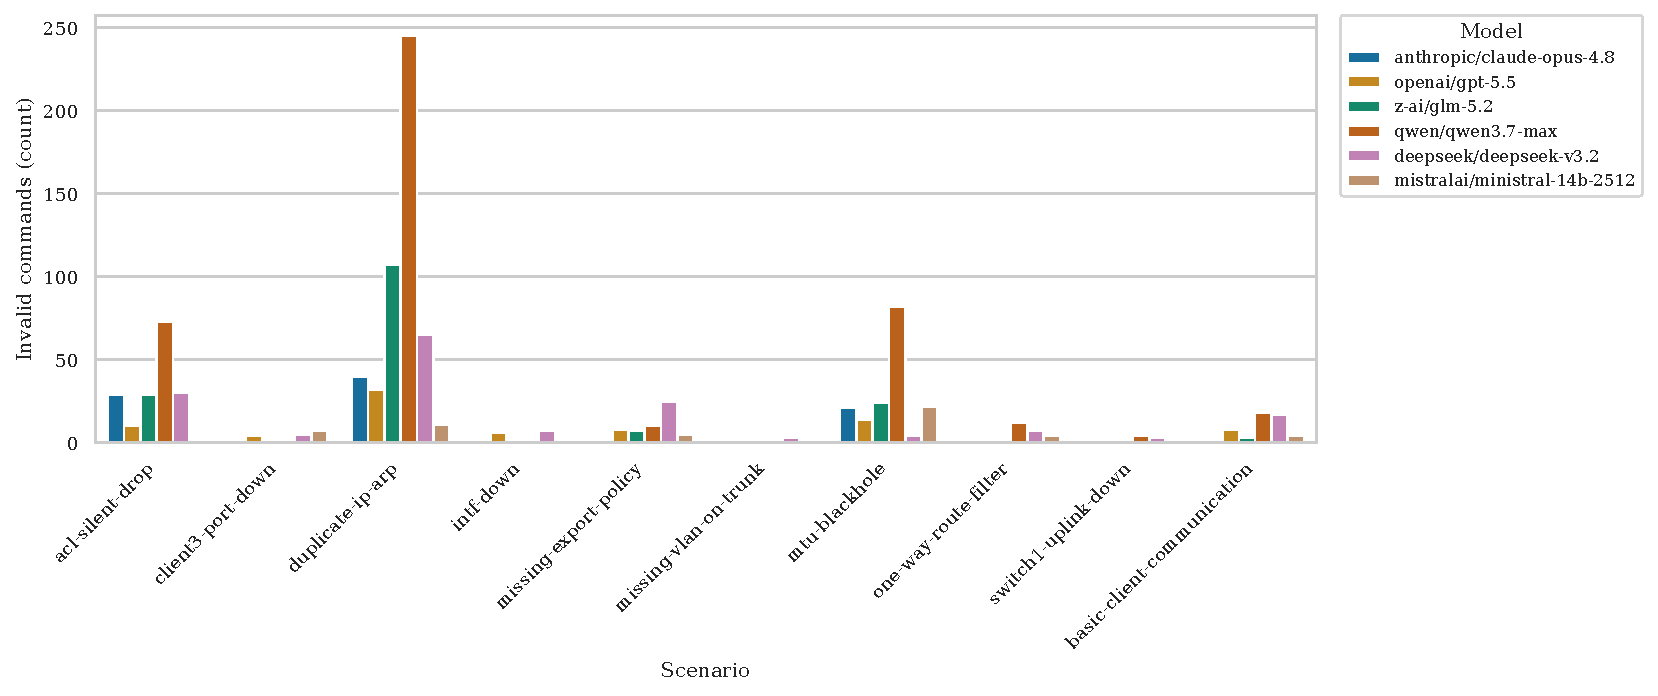
\includegraphics[width=\linewidth]{graphics/invalid_commands.pdf}
\end{center}
\caption{Malformed device commands per scenario and model.}
\label{fig:invalid-commands}
\end{figure}

\begin{figure}[htbp]
\begin{center}
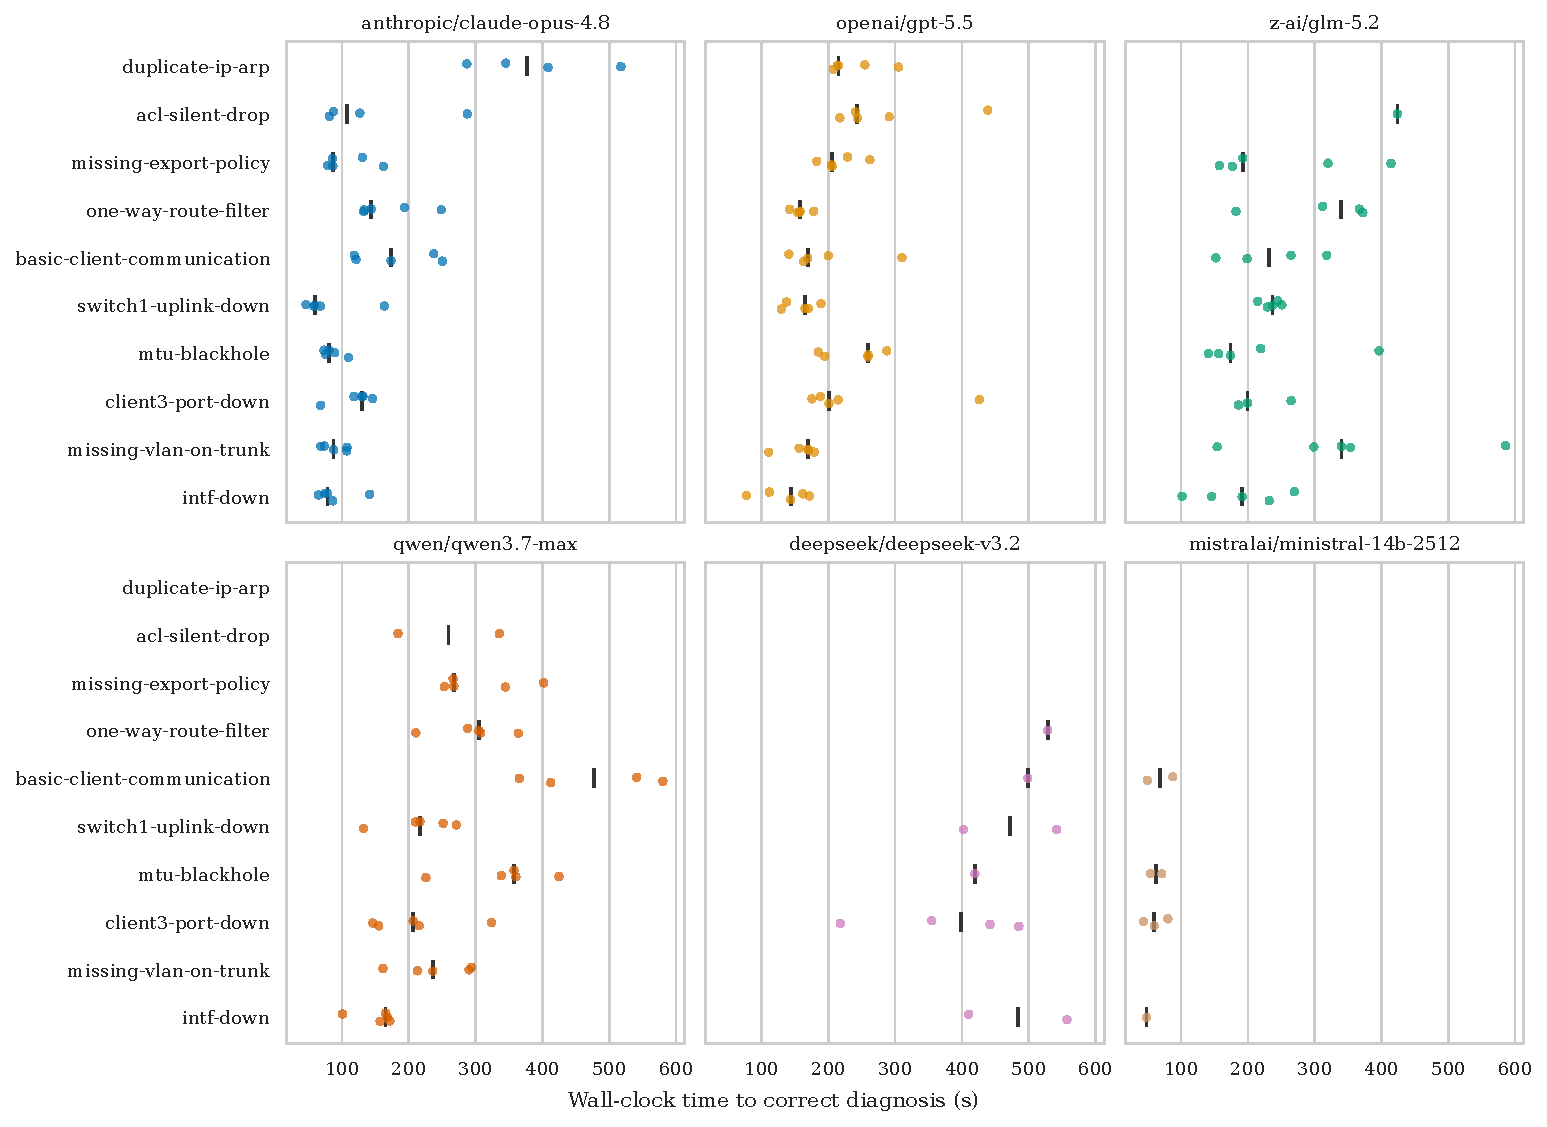
\includegraphics[width=0.8\linewidth]{graphics/scenario_time_to_diagnosis.pdf}
\end{center}
\caption{Wall-clock time to a correct diagnosis per scenario and model.}
\label{fig:scenario-ttd}
\end{figure}

\begin{figure}[htbp]
\begin{center}
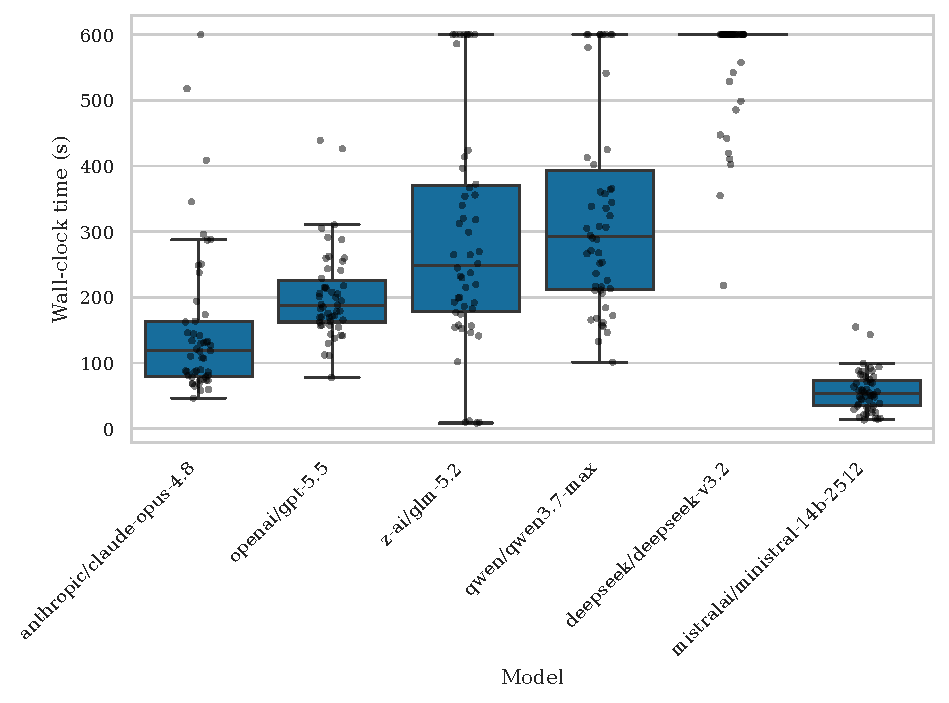
\includegraphics[width=0.85\linewidth]{graphics/distribution_wall_clock.pdf}
\end{center}
\caption{Wall-clock time per run over all 300 runs, including wrong diagnoses and DNFs.
Boxes show median and interquartile range. Dots are individual runs. The clusters at 600\,s
are the 55 runs stopped at the wall-clock cap.}
\label{fig:wall-clock-distribution}
\end{figure}

\clearpage
\subsection{User Interface Screenshots}
\label{app:ui-screenshots}

\Cref{fig:chat-interface} shows the web chat interface of \Cref{sec:impl-interfaces} in a troubleshooting scenario (a conversation).
\Cref{fig:investigation-status} shows the status page of the
autonomous syslog investigations (\Cref{sec:impl-investigations}). Each row is one automatically
opened case with its device, state and a summary of the findings. The detail view below lists the
triggering syslog event and the stored report of the selected case.

\begin{figure}[htbp]
\begin{center}
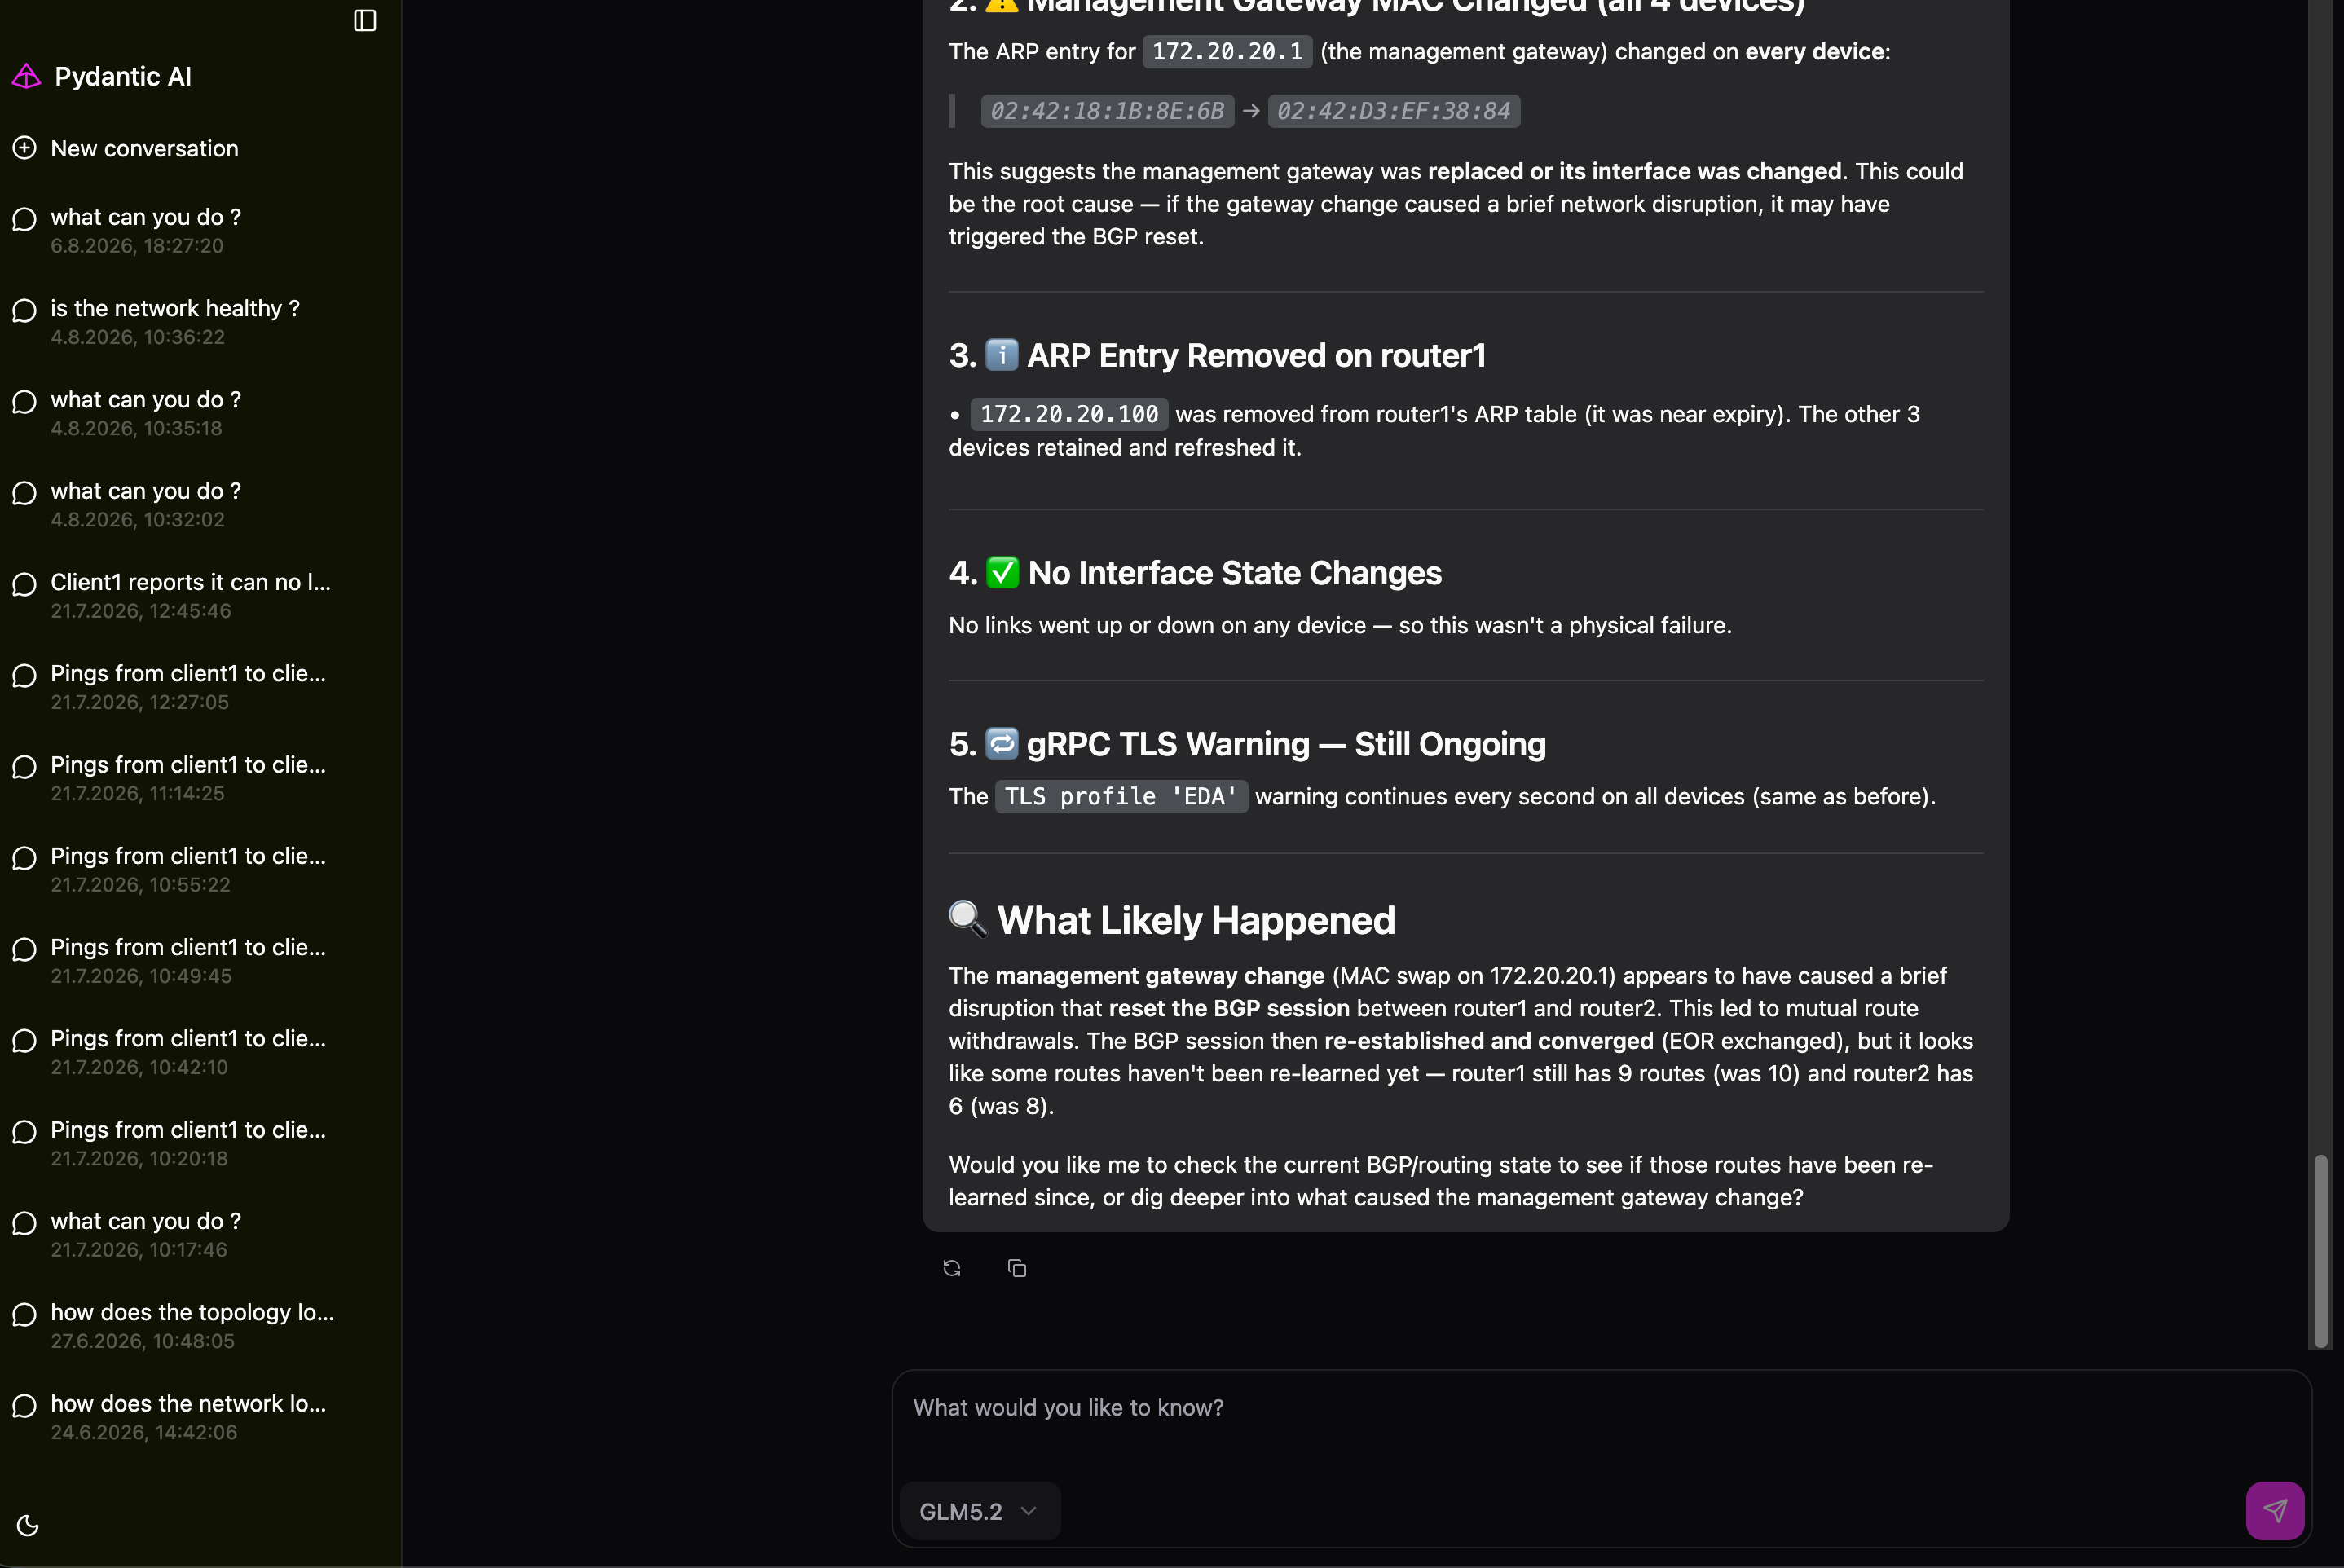
\includegraphics[width=\linewidth]{graphics/chat-interface.png}
\end{center}
\caption{The web chat interface with model selector, showing the closing answer of a
troubleshooting conversation.}
\label{fig:chat-interface}
\end{figure}

\begin{figure}[htbp]
\begin{center}
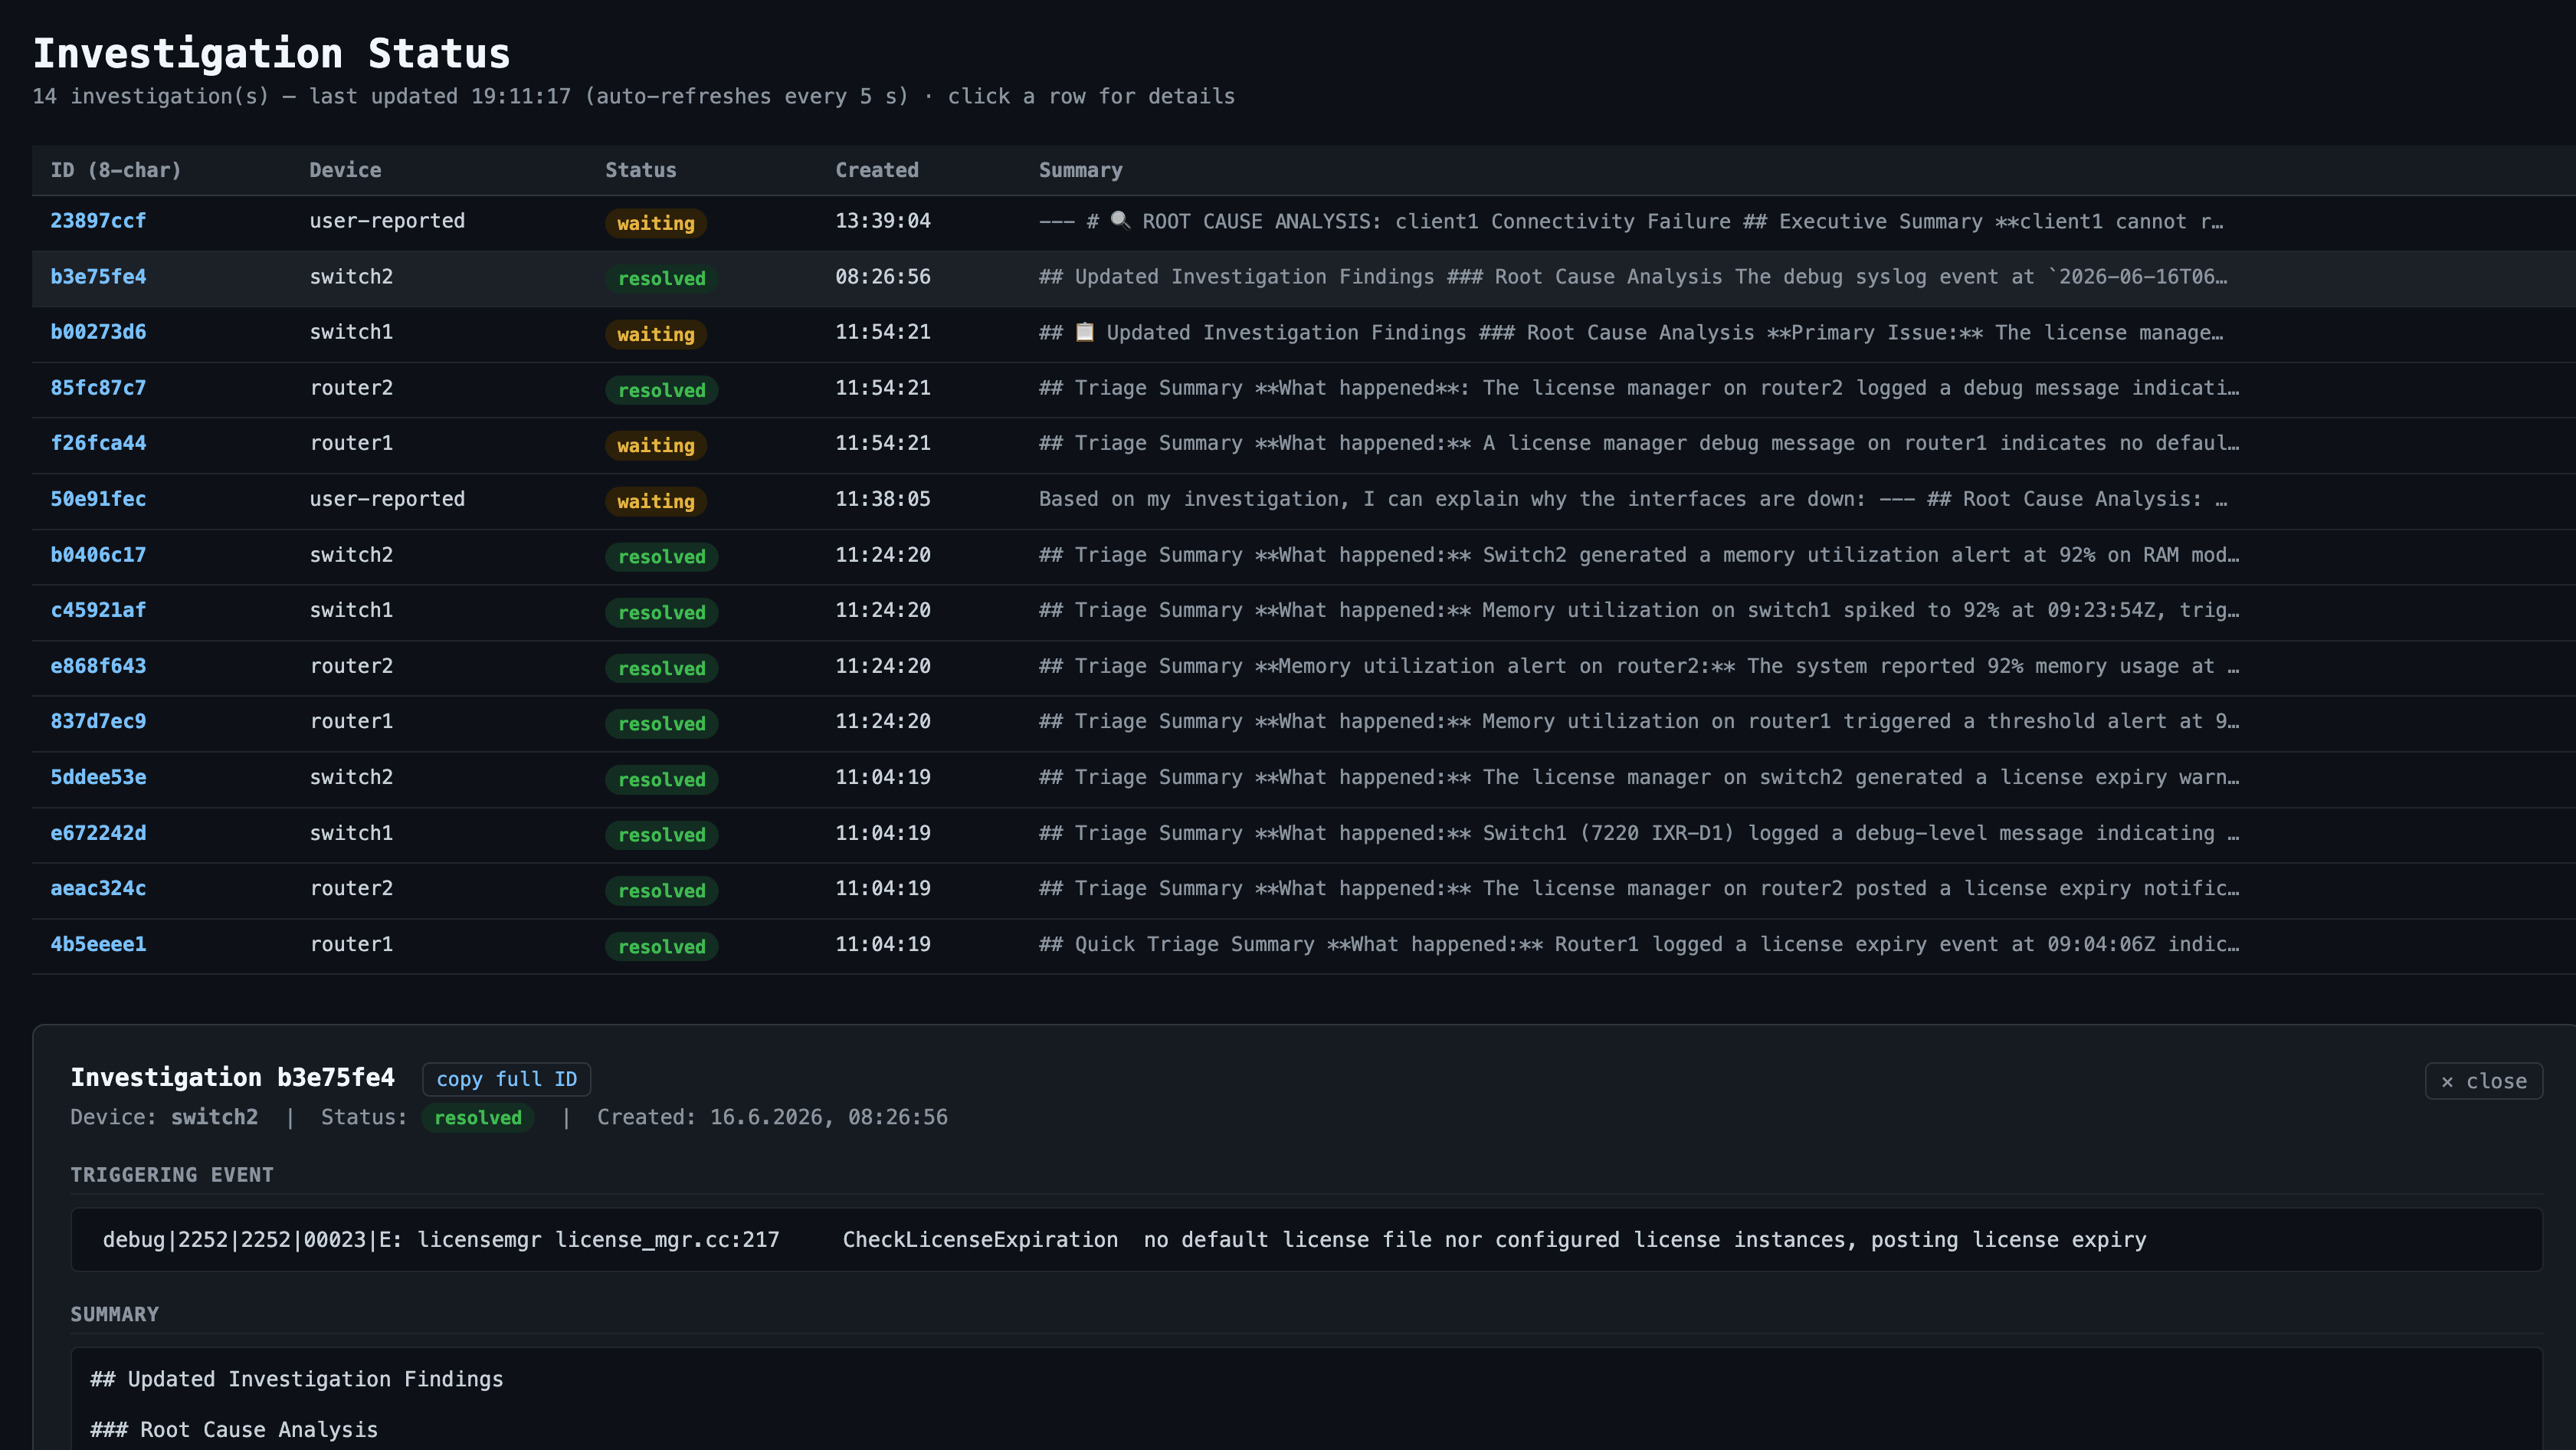
\includegraphics[width=\linewidth]{graphics/automatic-investigations.png}
\end{center}
\caption{The status page of the autonomous syslog investigations, with the list of open and
resolved cases and the detail view of one resolved investigation.}
\label{fig:investigation-status}
\end{figure}

\end{appendix}
